\documentclass[]{standalone}

\usepackage{graphicx}
\usepackage[linesnumbered,ruled,vlined]{algorithm2e}
\usepackage{color,soul}
\usepackage[utf8]{inputenc}
\usepackage[T1]{fontenc}
\usepackage{textcomp}
\usepackage{amsmath, amssymb}
\usepackage{caption}
\usepackage{listings}

% figure support
\usepackage{tikz}
\usetikzlibrary{calc}
\usepackage{import}
\usepackage{xifthen}
\pdfminorversion=7
\usepackage{pdfpages}
\usepackage{transparent}
\usepackage[hidelinks]{hyperref}

\pdfsuppresswarningpagegroup=1

\begin{document}
	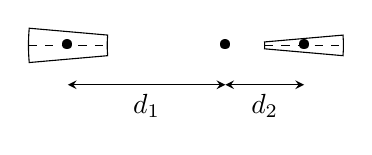
\begin{tikzpicture}[>=stealth]
		\def\angle{5}
		\node[] (Robot) at (0,0) {\textbullet};
		\node[] (A) at (1,0) {\textbullet};
		\node[] (B) at (-2,0) {\textbullet};
		\draw[dashed] (A)++(-0.5,0)--($(A)+(0.5,0)$);
		\draw[dashed] (B)++(-0.5,0)--($(B)+(0.5,0)$);

		\draw[] ($(Robot)+(\angle:1.5)$) arc (\angle:-\angle:1.5)
			--	($(Robot)+(-\angle:0.5)$) arc (-\angle:\angle:0.5)
			--	cycle ;

		\draw[] ($(Robot)+(180-\angle:1.5)$) arc (180-\angle:180+\angle:1.5)
			--	($(Robot)+(180+\angle:2.5)$) arc (180+\angle:180-\angle:2.5)
			--	cycle ;

		\draw[<->] ($(A)+(0,-0.5)$) -- ($(Robot)+(+0.0,-0.5)$);
		\draw[<->] ($(B)+(0,-0.5)$) -- ($(Robot)+(-0.0,-0.5)$);

		\node[below] (d1) at (-1,-0.5) {$d_1$};
		\node[below] (d2) at (0.5,-0.5) {$d_2$};
		
	\end{tikzpicture}
\end{document}
